\documentclass[10pt, a4paper]{article}
%Gummi|065|=)
\usepackage{graphicx}
\usepackage{CJK}
\usepackage{amsmath}
\usepackage{algorithm}
\usepackage[noend]{algpseudocode}
\begin{CJK}{UTF8}{gbsn}


\title{\textbf{Alogrithm exercise }}


\author{ywjia@mail.ustc.edu.cn\\
		SA14011066\\
		贾亚伟}
\date{2014-10-23}

\begin{document}

\maketitle
\DeclareGraphicsExtensions{.pdf,.png,.jpg}

\begin{center} 
\textbf{概率算法习题}
\end{center}
\section{ex1}
\textbf{程序ex1.c 见 ex 文件目录 }\\
\textbf{result as follows:} \\

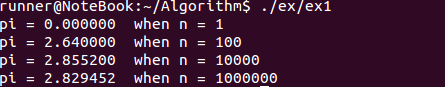
\includegraphics{../pic/ex1pic.png}

\section{ex2}
程序ex2.c 见 ex 文件目录  \\
\textbf{result as follows:} \\

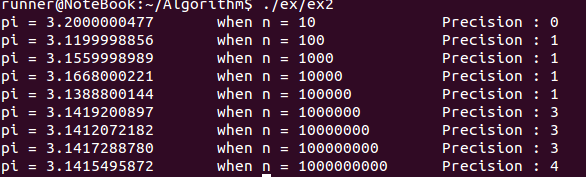
\includegraphics[width=15cm]{../pic/ex2.png}

\section{ex3}
\textbf{问题:}\\
 calculate the integer f: [a, b] $\rightarrow$ [c, d] \\
 here set f(x) = sin(x).\\
\textbf{程序ex3.c 见 ex 文件目录 } \\
\textbf{result as follows:} \\

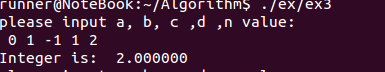
\includegraphics[width=15cm]{../pic/ex3.png}

\section{ex4}
\textbf{Question:} \\
Assume $\epsilon, \delta$ is constant within $(0, 1)$, prove: \\
If I is the correct value of $\int_0^1{f(x)dx}$, and h is the return value of alogrithm "HitorMiss", Then $Prob[|h-I| < \epsilon] \geq 1 - \delta$ when $n \geq I(1-I)/\epsilon^{2}\delta$. \\
 \textbf{Prove:}\\
Assume we hit the area n times and there are  k points scatterd under the area $f(x)$.Apparently, the random X that the number of points scattered under $f(x)$ is Binomial Distribution, that is $P_r(X = k) = C_n^{k}p^{k}(1-p)^{n-k}$
then, $E(X) = np, Var(X) = np(1-p)$.\\
the h that HitOrMiss return is $k/n$, So $h = X/n, E(h) = E(X/n) = p = k/n = I, Var(h) = Var(X/n) = \frac{p(1-p)}{n} = \delta^{2}$. \\
According to Chebyshev's inequality $Pr(|h - I| \leq \epsilon) \geq 1 - \delta^{2}/\epsilon^{2} $  And according to the cond: $n \geq I(1-I)/\epsilon^{2}\delta$, So we have $Pr(|h - I| \leq \epsilon )\geq 1 - \frac{p(1-p)}{\epsilon^{2}n} \geq 1 - \frac{p(1-p)}{\epsilon^{2}}\frac{\epsilon^{2}\delta}{I(1-I)} = 1 - \delta.\\
Q.E.D$

\section{ex5}

\textbf{程序ex5.py 见 ex 文件目录 }\\
\textbf{result as follows:} \\

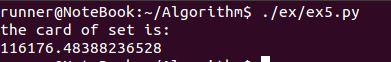
\includegraphics[width=15cm]{../pic/ex5.png}
\textbf{分析:} \\
实验结果表明,当要估值的集合的基越大,也就是$n$ 值越大 算法对n的估值越准确。
\section{ex6}

\textbf{问题:}
写一Sherwood算法C 与算法A,B,D比较,并给出实验结果。

\textbf{答案:} \\
程序ex6.c 见 ex 文件夹。 \\
程序运行结果如下:\\
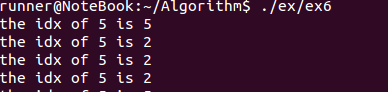
\includegraphics[width=15cm]{../pic/ex6.png}
\section{ex7}

\textbf{问题:} 
证明当放置第k+1个皇后时, 若有多个位置是开放的, 则算法QueensLV选中其中一位置的概率相等。


证: 假设在放置k+1个皇后时,有nb个位置可以放置, 并假设选中了第i个位置, 则其概率$p(i) = \frac{1}{i}\times\frac{i}{i+11}\times \cdots \times \frac{nb-1}{nb} = \frac{1}{nb}$ 即选中其中一个位置的概率均相等, 为$\frac{1}{nb}$。 

\section{ex8}

写一算法,求n=12-20时最优的StepVegas值。\\
\textbf{算法如下:}
\begin{algorithm}
\caption{求StepVegas最优值}\label{euclid}
\begin{algorithmic}[1]
\Procedure{OptimalStepVegas}{}
\State $\textit{mintime} \gets \infty$
\State $\textit{k} \gets 0$

\For{from $n = 12$ to  20 }
	\For{from $\textit{k} = 0$ to 20}
	\State $\textit{time} \gets QueensLv(n, success, \textit{k})$
	\If{$\textit{time} < \textit{mintime}$}
		\State $\textit{mintime} \gets \textit{time}$
		\State $\textit{stepVegas} \gets k$
 	\EndIf
 	\EndFor
 	
 	\State Print $The Count of Queens:n,  Optimal StepVegas Value is : stepVegas$
\EndFor

\EndProcedure
\end{algorithmic}
\end{algorithm}

\section{ex9}
\textbf{问题:打印10000 以内的素数并与确定性算法相比较,并给出100~10000以内错误的比
例。}
\textbf{解:}\\
程序ex9.c 见ex文件目录, 程序运行结果如下(部分):\\
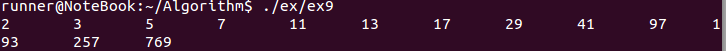
\includegraphics[width=15cm]{../pic/ex9.png}
错误比例为:(1204-845)/1204 = 29.5\% \\
 额,错误率有点高,但找了好久没找到原因~
\begin{center} 
\textbf{近似算法习题}
\end{center}
\section{完善证明}
\textbf{证:}
设最优调度使得每台机器恰有2个作业:Ji和Jj,则必有i≤m,j>m。否则若某最优调度O有i,j≤m,则定有某台机器上有Js和Jt,使得s,t>m.
   ∵Pi,Pj≥Ps,Pt,交换Pj和Pt,则
       Pi+Pt≤Pi+Pj         Ps+Pj≤Pi+Pj
交换后的调度O’的最迟完成时间只可能减少,故O’也是最优调度。对于i,j>m可类似证明。
∴必有最优调度使J1,...,Jm分别分配到M1,…,Mm上,当将Jm+1,...,J2m分配到M台机器上时,LPT是将长时间的作业分配到轻负载上,必与该最优调度结果相同。

\begin{center} 
\textbf{分布式算法习题}
\end{center}
\section{ex2.1}
\textbf{问题:}分析在同步和异步模型下,convergecast 算法的时间复杂性。\\
\textbf{答:}
1) 在同步模型中
最坏情况下,算法执行的每一轮中只有一个 msg 传递,而此时生成树汇聚最大
值的算法最多执行 $n-1$ 轮(即生成树中除了末端节点每一个节点只有一个子节
点),也就是说同步情况下时间复杂度为 $O(n-1)$\\
(2) 在异步模中
在异步模型的汇集算法的每个容许执行中,树中每个距离 $p_{r}$为 t 的处理器至多
在时刻 t 接收消息 M,因此对于每个节点而言,它到它所有子节点中 t 最大的
路径决定了它本身时间花费。因此在最坏情况下,仍应该是同步模型下的最坏
情况,即生成树中除了末端节点每一个节点只有一个子节点,此时时间复杂度
仍为 $O(n-1)$
\section{ex2.2}
\textbf{问题: G 里一结点从 pr 可达当且仅当它曾设置过自己的 parent 变量。}
 \textbf{证:}\\
 \textbf{必要性:}
因为图 G 是由 parent 和 children 确定的静态图,任一节点在收到 M 后才会加入到图
中。即可达节点收到过 M,执行了算法 2.2 的第五行。由于是容许执行的,所以第 7
行(parent:=j)也会执行。\\
\textbf{充分性:}一节点设置过自己的 parent 变量,则其从 $p_{r}$ 可达。
若算法 2.2 的第 7 行执行过了,因为是容许执行,则必然有第 5 行也执行过了。即节
点收到过 M。而 M 又是从 $p_{r}$ 发出的,所以该节点是从 $p_{r}$ 可达的。
\section{ex2.3}
\textbf{问题:}
证明 Alg2.3 构造一棵以 Pr 为根的 DFS 树。\\
\textbf{证:}\\
(1)算法 2.3 构造的图 G 必然是连通的。否则,设 G 存在邻居节点 $p_{j}$ 和 $p_{i}$。$p_{j}$ 从 $p_{r}$ 可
达,但 $p_{i}$ 从 $p_{r}$ 是不可达的。
则:\\
1) $p_{i}$ 的 parent 为空;\\
2) $p_{i}$ 不为 $p_{j}$ 的 child.\\
因为:
G 里一结点从 $p_{r}$ 可达当且仅当它曾设置过自己的 parent 变量。
所以:\\
1) $p_{j}$ 的 parent 必然设置过了;\\
2) $p_{i}$ 的 parent 为 nill;\\
3) $p_{i}$ 属于 $p_{j}$ 的 unexplored 集合。\\
而算法的第 11 和 14 行决定了 $p_{j}$ 会向 $p_{i}$ 发送 M,使得 $p_{i}$ 的 parent 成为 $p_{j}$,$p_{i}$ 成为 $p_{j}$
的 child。
这与假设的结果矛盾。故$p_{i}$ 必然也是从 $p_{r}$可达的。\\
(2)算法 2.3 构造的图 G 必然是无环的。否则设 G 中有一个环, $p_{1}$,$p_{2}$,...,$p_{i}$, $p_{1}$。令 $p_{1}$ 是
该环中最早接收到 M 的节点。则 $p_{i}$ 是从 $p_{1}$ 可达的,且 $p_{1}$ 的 parent 是 $p_{i}$,$p_{1}$ 是 $p_{i}$
的 child。
而 $p_{i}$ 在收到 M 后,向 $p_{1}$ 发送 M。因为 $p_{1}$ 的 parent 已经不为空,所以 $p_{1}$ 收到来自
$p_{i}$ 的 M 时,根据第 16 行代码,$p_{1}$ 会向 $p_{i}$ 放回一个$<reject>$信息,不会将 $p_{i}$ 设为
parent。而 $p_{i}$ 未收到 $p_{1}$ 返回的<parent>信息,也不会将 $p_{1}$ 设为 child。与前面的出
的结果矛盾。
故 G 是无环的。\\
(3) 图 G 是一棵 DFS 树。只需证明在有子结点与兄弟结点未访问时,子结点总是先加入
树中。
设有节点 $p_{1}$,$p_{2}$ 和 $p_{3}$。$p_{2}$ 和 $p_{3}$ 是 $p_{1}$ 的直接相邻节点。$p_{1}$ 在第 12~14 行中先选择
向 $p_{2}$ 发送 M,则 $p_{1}$ 当且仅当 $p_{2}$ 向其返回一个$<parent>$(第 17 行,第 22 行)时才
有可能向 $p_{3}$ 发送 M。
而 $p_{2}$ 仅在其向所有的相邻节点发送过 M 后才会向 $p_{1}$ 返回$<parent>$ (第 19~21 行)。
所以 $p_{2}$ 的子节点是永远先于 $p_{3}$ 加入树中的,即 G 是 DFS 树。
\section{ex2.4}
\textbf{问题:证明 Alg2.3 的时间复杂性为 O(m)}\\
\textbf{证明:}\\
1):同步模型:每一轮中,根据算法,有且只有一个消息(M or Parent or Reject)在传输,
从算法的第 6 、14、16、20、25 行发送消息的语句中可以发现:消息只发往一个处理
器结点,除根结点外,所有的处理器都是收到消息后才被激活,所以,不存在多个处
理器在同一轮发送消息的情况,所以时间复杂度与消息复杂度一致。\\
(2)异步模型:在一个时刻内至多有一个消息在传输,因此,时间复杂度也与消息复杂度
一致。消息复杂度:对任一边,可能传输的消息最多有 4 个,即 2 个 M ,2 个相应 M
的消息(Parent or Reject)
,所以消息复杂度为 O(m)
综上,该算法的时间复杂度为 O(m)

\section{ex2.5}
\textbf{问题:修改 Alg2.3 获得一新算法,使构造 DFS 树的时间复杂性为 O(n)。}\\
\textbf{解:}\\
(1)在每个处理器中维护一本地变量,同时添加一消息类型,在处理器 Pi 转发 M 时,发
送消息 N 通知其余的为访问过的邻居,这样其邻居在转发 M 时便不会向 Pi 转发。\\
(2)在消息 M 和<parent>中维护一发送数组,记录已经转发过 M 的处理器名称。
两种方式都是避免向已转发过 M 的处理器发送消息 M,这样 DFS 树外的边不再耗时,
时间。
复杂度也降为 O(n)

\section{ex3.1}
\textbf{问题:证明同步环系统中不存在匿名的、一致性的领导者选举算法。}\\
\textbf{解:}\\
在匿名系统中,每个处理器在系统中具有相同的状态机。由 Lemma3.1 可知,设算法 A 是使
环上某个处理器为 leader 的算法。因为环是同步的,且只有一种初始配置。在每轮里,各处
理器均发出同样的 message,所以在各轮里各个处理器接收到相同的 message,则状态改变也
相同。所以所有处理要么同为 leader,要么同时不为 leader。
故同步环系统中匿名的、一致性的领导者选举算法的算法是不存在的。
\section{ex3.2}
\textbf{问题:证明异步环系统中不存在匿名的领导者选举算法。}\\
\textbf{解:}\\
每个处理器的初始状态和状态机相同,除了接收消息的时间可能不同外,接收到的消息序列
也相同。所以最终处理器的状态也是一致的。由于处理器处理一条消息至多需要 1 单位时间,若某时刻某个处理器宣布自己是 leader,则在有限时间内,其它处理器也会宣布自己是 leader。故异步环系统中匿名的领导者选举算法是不存在的。

\section{ex3.9}
\textbf{问题:若将环 $R^{rev}$ 划分为长度为 j(j 是 2 的方幂)的连续片段,则所有这些片段是次序等价的.}\\
\textbf{解:}\\
对一个整数$P,(0 \leq P \leq n-1)$ 可以表示为: $P = \sum_{i=1}^{m}a_{i}2^{i-1}$, 其中 $m = \log n$, 则有$rev(P) = \sum_{i=1}^{m}a_{i}2^{i-1}$\\
设 $P, Q$ 在同一个片段上, $P_{1}, Q_{1}$在同一片段上, 且设这两个片段是相邻, 由模运算的加法可得:\\
$P_{1} = P + l \\Q_{1} = Q+l$ 式中l表示片段的长度, $l = 2^{k}$. 另:\\
$$P = \sum_{i=1}^{m}a_{i}2^{i-1}$$ $$ Q = \sum_{i=1}^{m}a_{i}2^{i-1}$$  且 P,Q 在同一片段上有 $|P-Q| \le 1 = 2^{k}$ 所以存在 $r(0 \leq r \leq k)$, 满足$a_{r} \neq b_{r}$. 否则, $|P-Q| \ \geq 1$. 这与P, Q 在同一个片段上矛盾。\\
设$s = min{r}$, 则根据 rev(P), rev(Q)的表示方法可得:$$sign() rev(P)- rev(Q) = sign(a-b)$$ 而 $$P_{1}= P+1 = \sum_{i=1}^{m}a_{i}2^{i-1} + 2^{k}$$ $$Q_{1}= Q+1 = \sum_{i=1}^{m}a_{i}2^{i-1} + 2^{k}$$ 显然, P 与$P_{1}$ 的前k位相同,Q 与$Q_{1}$ 的前k位相同。 由$0 \leq s \leq k$ 得$$sign() rev(P)- rev(Q) = sign(a-b)$$ 这两个相邻片段是序等价的,根据等价的传递关系,可得所有的片段都是次序等价的。

\end{CJK}
\end{document}

